\documentclass{tufte-book}%[a4paper,twoside]
% See https://github.com/Tufte-LaTeX/tufte-latex/blob/master/sample-book.tex for details

\title{Alice in Bitcoinland}
\author{Gigi}
\publisher{Do I Really Need a Publisher}

% Packages
\usepackage{lipsum}
\usepackage{booktabs}
\usepackage{graphicx}
\setkeys{Gin}{width=\linewidth,totalheight=\textheight,keepaspectratio}
\graphicspath{{graphics/}}

%%
% Just some sample text
\usepackage{lipsum}

%%
% For nicely typeset tabular material
\usepackage{booktabs}

%%
% For graphics / images
\usepackage{graphicx}
\setkeys{Gin}{width=\linewidth,totalheight=\textheight,keepaspectratio}
\graphicspath{{graphics/}}

% The fancyvrb package lets us customize the formatting of verbatim
% environments.  We use a slightly smaller font.
\usepackage{fancyvrb}
\fvset{fontsize=\normalsize}

%%
% Prints argument within hanging parentheses (i.e., parentheses that take
% up no horizontal space).  Useful in tabular environments.
\newcommand{\hangp}[1]{\makebox[0pt][r]{(}#1\makebox[0pt][l]{)}}

%%
% Prints an asterisk that takes up no horizontal space.
% Useful in tabular environments.
\newcommand{\hangstar}{\makebox[0pt][l]{*}}

%%
% Prints a trailing space in a smart way.
\usepackage{xspace}

%%
% Some shortcuts for Tufte's book titles.  The lowercase commands will
% produce the initials of the book title in italics.  The all-caps commands
% will print out the full title of the book in italics.
\newcommand{\vdqi}{\textit{VDQI}\xspace}
\newcommand{\ei}{\textit{EI}\xspace}
\newcommand{\ve}{\textit{VE}\xspace}
\newcommand{\be}{\textit{BE}\xspace}
\newcommand{\VDQI}{\textit{The Visual Display of Quantitative Information}\xspace}
\newcommand{\EI}{\textit{Envisioning Information}\xspace}
\newcommand{\VE}{\textit{Visual Explanations}\xspace}
\newcommand{\BE}{\textit{Beautiful Evidence}\xspace}

\newcommand{\TL}{Tufte-\LaTeX\xspace}

% Prints the month name (e.g., January) and the year (e.g., 2008)
\newcommand{\monthyear}{%
  \ifcase\month\or January\or February\or March\or April\or May\or June\or
  July\or August\or September\or October\or November\or
  December\fi\space\number\year
}


% Prints an epigraph and speaker in sans serif, all-caps type.
\newcommand{\openepigraph}[2]{%
  %\sffamily\fontsize{14}{16}\selectfont
  \begin{fullwidth}
  \sffamily\large
  \begin{doublespace}
  \noindent\allcaps{#1}\\% epigraph
  \noindent\allcaps{#2}% author
  \end{doublespace}
  \end{fullwidth}
}

% Inserts a blank page
\newcommand{\blankpage}{\newpage\hbox{}\thispagestyle{empty}\newpage}

\usepackage{units}

% Typesets the font size, leading, and measure in the form of 10/12x26 pc.
\newcommand{\measure}[3]{#1/#2$\times$\unit[#3]{pc}}

% Macros for typesetting the documentation
\newcommand{\hlred}[1]{\textcolor{Maroon}{#1}}% prints in red
\newcommand{\hangleft}[1]{\makebox[0pt][r]{#1}}
\newcommand{\hairsp}{\hspace{1pt}}% hair space
\newcommand{\hquad}{\hskip0.5em\relax}% half quad space
\newcommand{\TODO}{\textcolor{red}{\bf TODO!}\xspace}
\newcommand{\na}{\quad--}% used in tables for N/A cells
\providecommand{\XeLaTeX}{X\lower.5ex\hbox{\kern-0.15em\reflectbox{E}}\kern-0.1em\LaTeX}
\newcommand{\tXeLaTeX}{\XeLaTeX\index{XeLaTeX@\protect\XeLaTeX}}
% \index{\texttt{\textbackslash xyz}@\hangleft{\texttt{\textbackslash}}\texttt{xyz}}
\newcommand{\tuftebs}{\symbol{'134}}% a backslash in tt type in OT1/T1
\newcommand{\doccmdnoindex}[2][]{\texttt{\tuftebs#2}}% command name -- adds backslash automatically (and doesn't add cmd to the index)
\newcommand{\doccmddef}[2][]{%
  \hlred{\texttt{\tuftebs#2}}\label{cmd:#2}%
  \ifthenelse{\isempty{#1}}%
    {% add the command to the index
      \index{#2 command@\protect\hangleft{\texttt{\tuftebs}}\texttt{#2}}% command name
    }%
    {% add the command and package to the index
      \index{#2 command@\protect\hangleft{\texttt{\tuftebs}}\texttt{#2} (\texttt{#1} package)}% command name
      \index{#1 package@\texttt{#1} package}\index{packages!#1@\texttt{#1}}% package name
    }%
}% command name -- adds backslash automatically
\newcommand{\doccmd}[2][]{%
  \texttt{\tuftebs#2}%
  \ifthenelse{\isempty{#1}}%
    {% add the command to the index
      \index{#2 command@\protect\hangleft{\texttt{\tuftebs}}\texttt{#2}}% command name
    }%
    {% add the command and package to the index
      \index{#2 command@\protect\hangleft{\texttt{\tuftebs}}\texttt{#2} (\texttt{#1} package)}% command name
      \index{#1 package@\texttt{#1} package}\index{packages!#1@\texttt{#1}}% package name
    }%
}% command name -- adds backslash automatically
\newcommand{\docopt}[1]{\ensuremath{\langle}\textrm{\textit{#1}}\ensuremath{\rangle}}% optional command argument
\newcommand{\docarg}[1]{\textrm{\textit{#1}}}% (required) command argument
\newenvironment{docspec}{\begin{quotation}\ttfamily\parskip0pt\parindent0pt\ignorespaces}{\end{quotation}}% command specification environment
\newcommand{\docenv}[1]{\texttt{#1}\index{#1 environment@\texttt{#1} environment}\index{environments!#1@\texttt{#1}}}% environment name
\newcommand{\docenvdef}[1]{\hlred{\texttt{#1}}\label{env:#1}\index{#1 environment@\texttt{#1} environment}\index{environments!#1@\texttt{#1}}}% environment name
\newcommand{\docpkg}[1]{\texttt{#1}\index{#1 package@\texttt{#1} package}\index{packages!#1@\texttt{#1}}}% package name
\newcommand{\doccls}[1]{\texttt{#1}}% document class name
\newcommand{\docclsopt}[1]{\texttt{#1}\index{#1 class option@\texttt{#1} class option}\index{class options!#1@\texttt{#1}}}% document class option name
\newcommand{\docclsoptdef}[1]{\hlred{\texttt{#1}}\label{clsopt:#1}\index{#1 class option@\texttt{#1} class option}\index{class options!#1@\texttt{#1}}}% document class option name defined
\newcommand{\docmsg}[2]{\bigskip\begin{fullwidth}\noindent\ttfamily#1\end{fullwidth}\medskip\par\noindent#2}
\newcommand{\docfilehook}[2]{\texttt{#1}\index{file hooks!#2}\index{#1@\texttt{#1}}}
\newcommand{\doccounter}[1]{\texttt{#1}\index{#1 counter@\texttt{#1} counter}}

% Generates the index
\usepackage{makeidx}
\makeindex

\begin{document}

\frontmatter

\maketitle

\cleardoublepage


%%
% Start the main matter (normal chapters)
\mainmatter

\chapter*{Einleitung}
\label{ch:introduction}

\begin{chapquote}{Lewis Carroll, \textit{Alice im Wunderland}}
\enquote{Aber ich möchte nicht unter verrückte Leute geraten,} bemerkte Alice.
\enquote{Oh, da kommst du nicht drum herum,} sagte die Katze: \enquote{Wir sind
hier alle verrückt. Ich bin verrückt. Du bist verrückt.} \enquote{Woher weißt
du, daß ich verrückt bin?} sagte Alice. \enquote{du mußt es sein,} sagte die
Katze, \enquote{sonst wärst du nicht hergekommen.}
\end{chapquote}

Im Oktober 2018 stellte Arjun Balaji die harmlose Frage: \textit{Was hast du von
Bitcoin gelernt?} Nachdem ich versucht hatte, diese Frage in einem kurzen Tweet
zu beantworten, und kläglich scheiterte, wurde mir klar, dass die Dinge, die ich
gelernt habe viel zu zahlreich sind, um sie schnell oder überhaupt zu
beantworten.

Die Dinge, die ich gelernt habe, sind offensichtlich auf Bitcoin bezogen – oder
stehen zumindest im Zusammenhang damit. Obwohl einige der inneren Funktionen von
Bitcoin am Rande erklärt werden, sind die folgenden Lektionen keine Erklärung
dafür, wie Bitcoin funktioniert oder was es ist. Sie könnten jedoch helfen,
einige der Dinge zu erkunden, die Bitcoin berührt: philosophische Fragen,
wirtschaftliche Gegebenheiten und technologische Innovationen.

\begin{center}
  
\includegraphics[width=7cm]{assets/images/the-tweet.png}
\end{center}

Die \textit{21 Lektionen} sind in Siebener-Bündel gegliedert, was letztendlich
zu drei Teilen führt. Jeder Teil betrachtet Bitcoin durch eine
unterschiedliche Linse und zeigt, welche Erkenntnisse daraus gezogen werden
können, wenn man dieses seltsame Netzwerk aus einem anderen Blickwinkel
betrachtet.

\paragraph{\hyperref[ch:philosophy]{Teil I}} untersucht die philosophischen
Lehren von Bitcoin. Das Zusammenspiel von Unveränderlichkeit und Veränderung,
das Konzept der wahren Knappheit, Bitcoins unbefleckte Empfängnis, das Problem
der Identität, der Widerspruch von Replikation und Lokalität, die Macht der freien
Meinungsäußerung und die Grenzen des Wissens.

\paragraph{\hyperref[ch:economics]{Teil II}} untersucht die wirtschaftlichen
Lehren von Bitcoin. Lektionen über finanzielle Unwissenheit, Inflation, Wert,
Geld und die Geschichte des Geldes, Mindestreserve-Bankensystem und wie Bitcoin
auf raffinierte und kuriose Weise wieder gesundes bzw. solides Geld auf den
Markt bringt.

\paragraph{\hyperref[ch:technology]{Teil III}} untersucht einige der Lehren, die
aus der Auseinandersetzung mit der Technologie von Bitcoin hervorgegangen sind.
Warum Stärke in Zahlen zu finden ist, was Vertrauen bedeutet, warum das
Messen von Zeit arbeitsintensiv ist, warum behutsames Fortbewegen ein Feature
und kein Bug ist, was die Erschaffung von Bitcoin uns über die Privatsphäre
vermitteln kann, warum Cypherpunks Code schreiben (und nicht Gesetze) und welche
Metaphern nützlich sein könnten, um die Zukunft von Bitcoin zu erforschen.

~

Jede Lektion enthält mehrere Zitate und Links im gesamten Text. Wenn du tiefer
in die Materie eintauchen möchtest, findest du Links zu den wichtigsten
Materialien in den Fußnoten und in den Quellenangaben am Ende des Buches.

Auch wenn einige Vorkenntnisse über Bitcoin von Vorteil sind, hoffe ich, dass
diese Lektionen von jedem interessierten Leser verinnerlicht werden können.
Während einige sich aufeinander beziehen, sollte jede Lektion für sich allein
stehen und unabhängig voneinander gelesen werden können. Ich habe mein Bestes
getan, um mich vor Fachjargon zu scheuen, auch wenn einige domänenspezifische
Vokabeln unvermeidlich sind.

Ich hoffe, dass mein Schreiben anderen als Inspiration dient etwas tiefer
zu graben und einige der weitgreiferenden Fragen zu untersuchen welche Bitcoin
aufwirft. Meine eigene Inspiration kam von einer Vielzahl von Autoren, Bloggern,
und anderen kreativen Köpfen aus dem Internet, welchen ich ewig dankbar bin.

Zu guter Letzt: Mir geht es nicht darum dich, lieber Leser, von irgendetwas zu
überzeugen. Mein Ziel ist es dich zum Nachdenken zu bringen und dir zu zeigen,
dass hinter Bitcoin mehr steckt als man denkt. Ich kann dir gar nicht sagen,
was Bitcoin ist oder was Bitcoin dir beibringen wird. Das musst du selbst
herausfinden.

\begin{quotation}\begin{samepage}
\enquote{Danach gibt es kein Zurück mehr. Du nimmst die blaue Pille --- die
Geschichte endet hier, du wachst in deinem Bett auf und glaubst, was du glauben
willst. Du nimmst die rote Pille\footnote{die \textit{orange} Pille} --- du
bleibst im Wunderland, und ich zeige dir, wie weit der Kaninchenbau reicht.}
\begin{flushright} -- Morpheus
\end{flushright}\end{samepage}\end{quotation}

\begin{figure}
  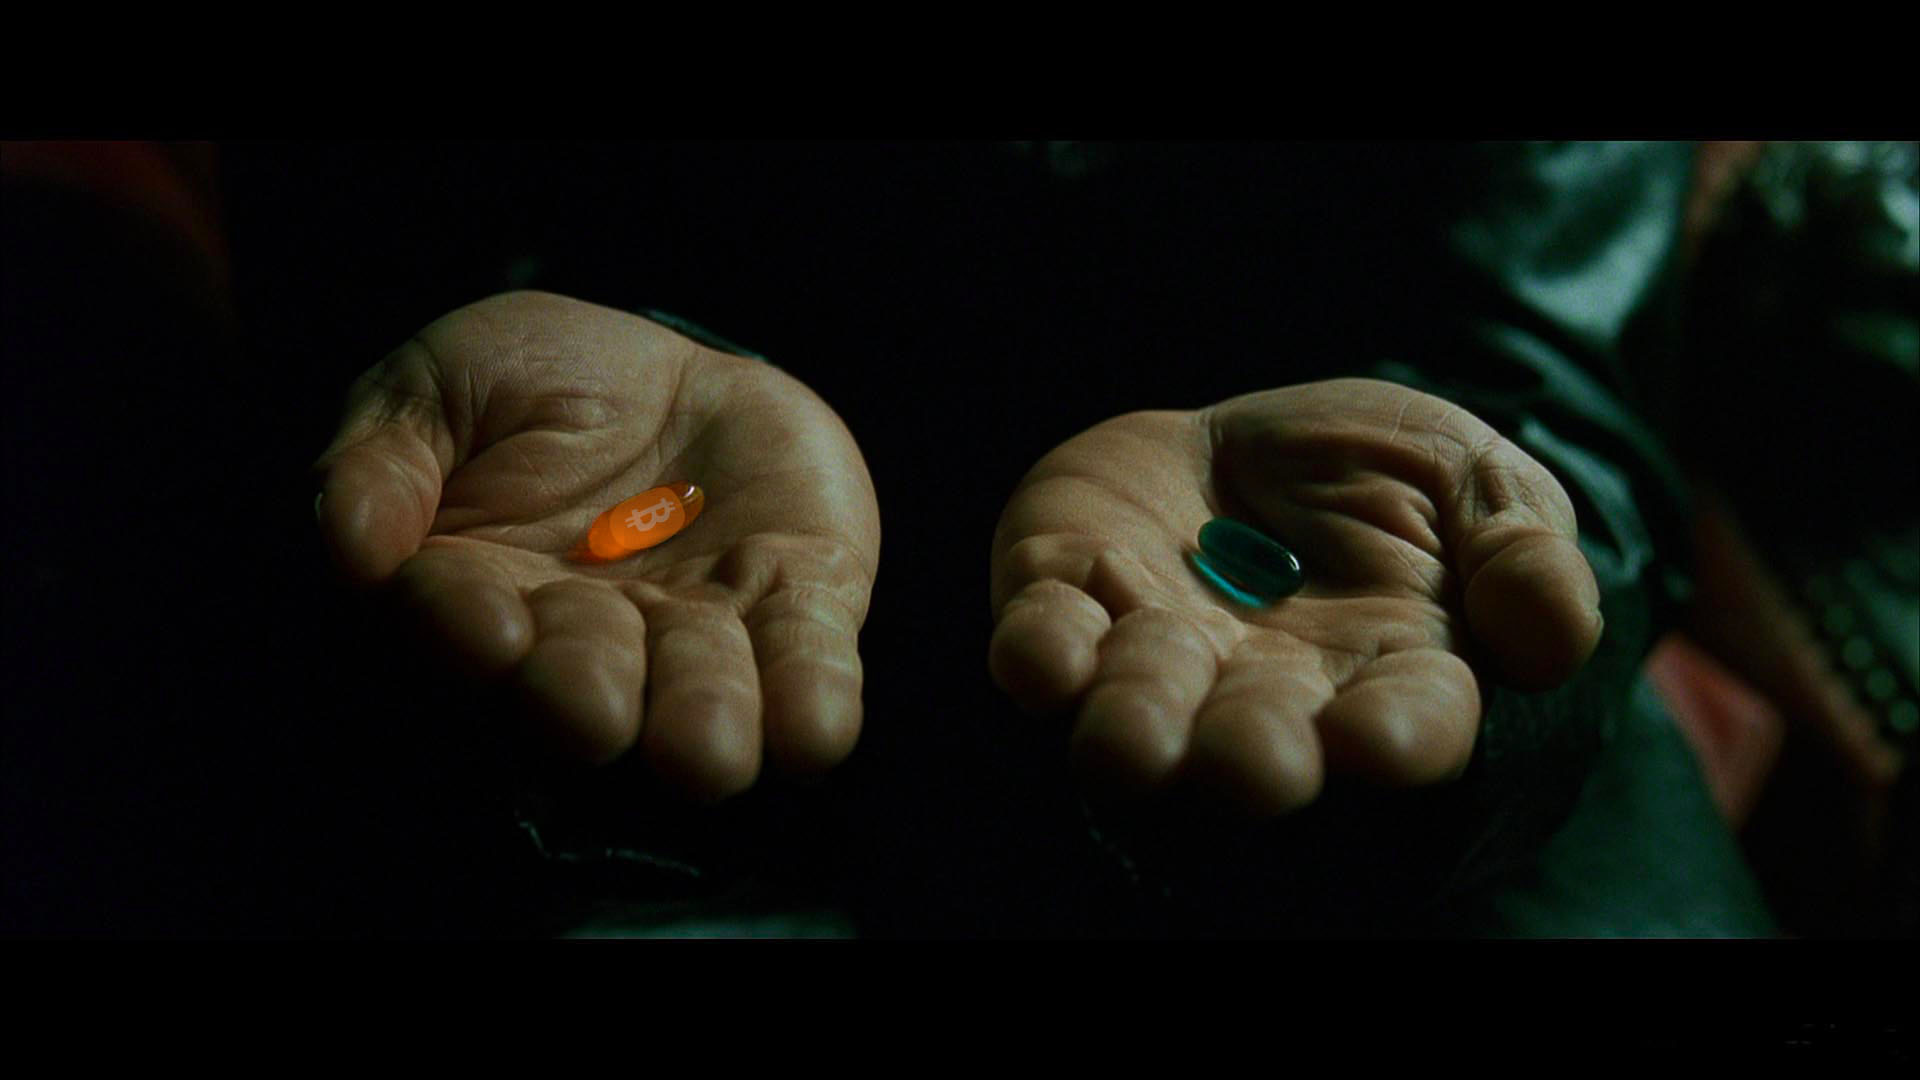
\includegraphics[width=\textwidth]{assets/images/bitcoin-orange-pill.jpg}
  \caption*{Bedenke! Alles, was ich dir anbiete, ist die Wahrheit. Nicht mehr.}
  \label{fig:bitcoin-orange-pill}
\end{figure}

%
% [Morpheus]: https://en.wikipedia.org/wiki/Red_pill_and_blue_pill#The_Matrix_(1999)
% [this question]: https://twitter.com/arjunblj/status/1050073234719293440
%
% <!-- Internal -->
% [chapter1]: {{ 'bitcoin/lessons/ch1-00-philosophy' | absolute_url }}
% [chapter2]: {{ 'bitcoin/lessons/ch2-00-economics' | absolute_url }}
% [chapter3]: {{ 'bitcoin/lessons/ch3-00-technology' | absolute_url }}
%
% <!-- Wikipedia -->
% [alice]: https://en.wikipedia.org/wiki/Alice%27s_Adventures_in_Wonderland
% [carroll]: https://en.wikipedia.org/wiki/Lewis_Carroll

\part{Philosophy}
\label{ch:philosophy}
\chapter*{Philosophy}

\begin{chapquote}{Lewis Carroll, \textit{Alice in Wonderland}}
The mouse looked at her rather inquisitively, and seemed to her to wink with one
of its little eyes, but it said nothing.
\end{chapquote}

Looking at Bitcoin superficially, one might conclude that it is slow, wasteful,
unnecessarily redundant, and overly paranoid. Looking at Bitcoin inquisitively,
one might find out that things are not as they seem at first glance.

Bitcoin has a way of taking your assumptions and turning them on their heads.
After a while, just when you were about to get comfortable again, Bitcoin will
smash through the wall like a bull in a china shop and shatter your assumptions
once more.

\begin{figure}
  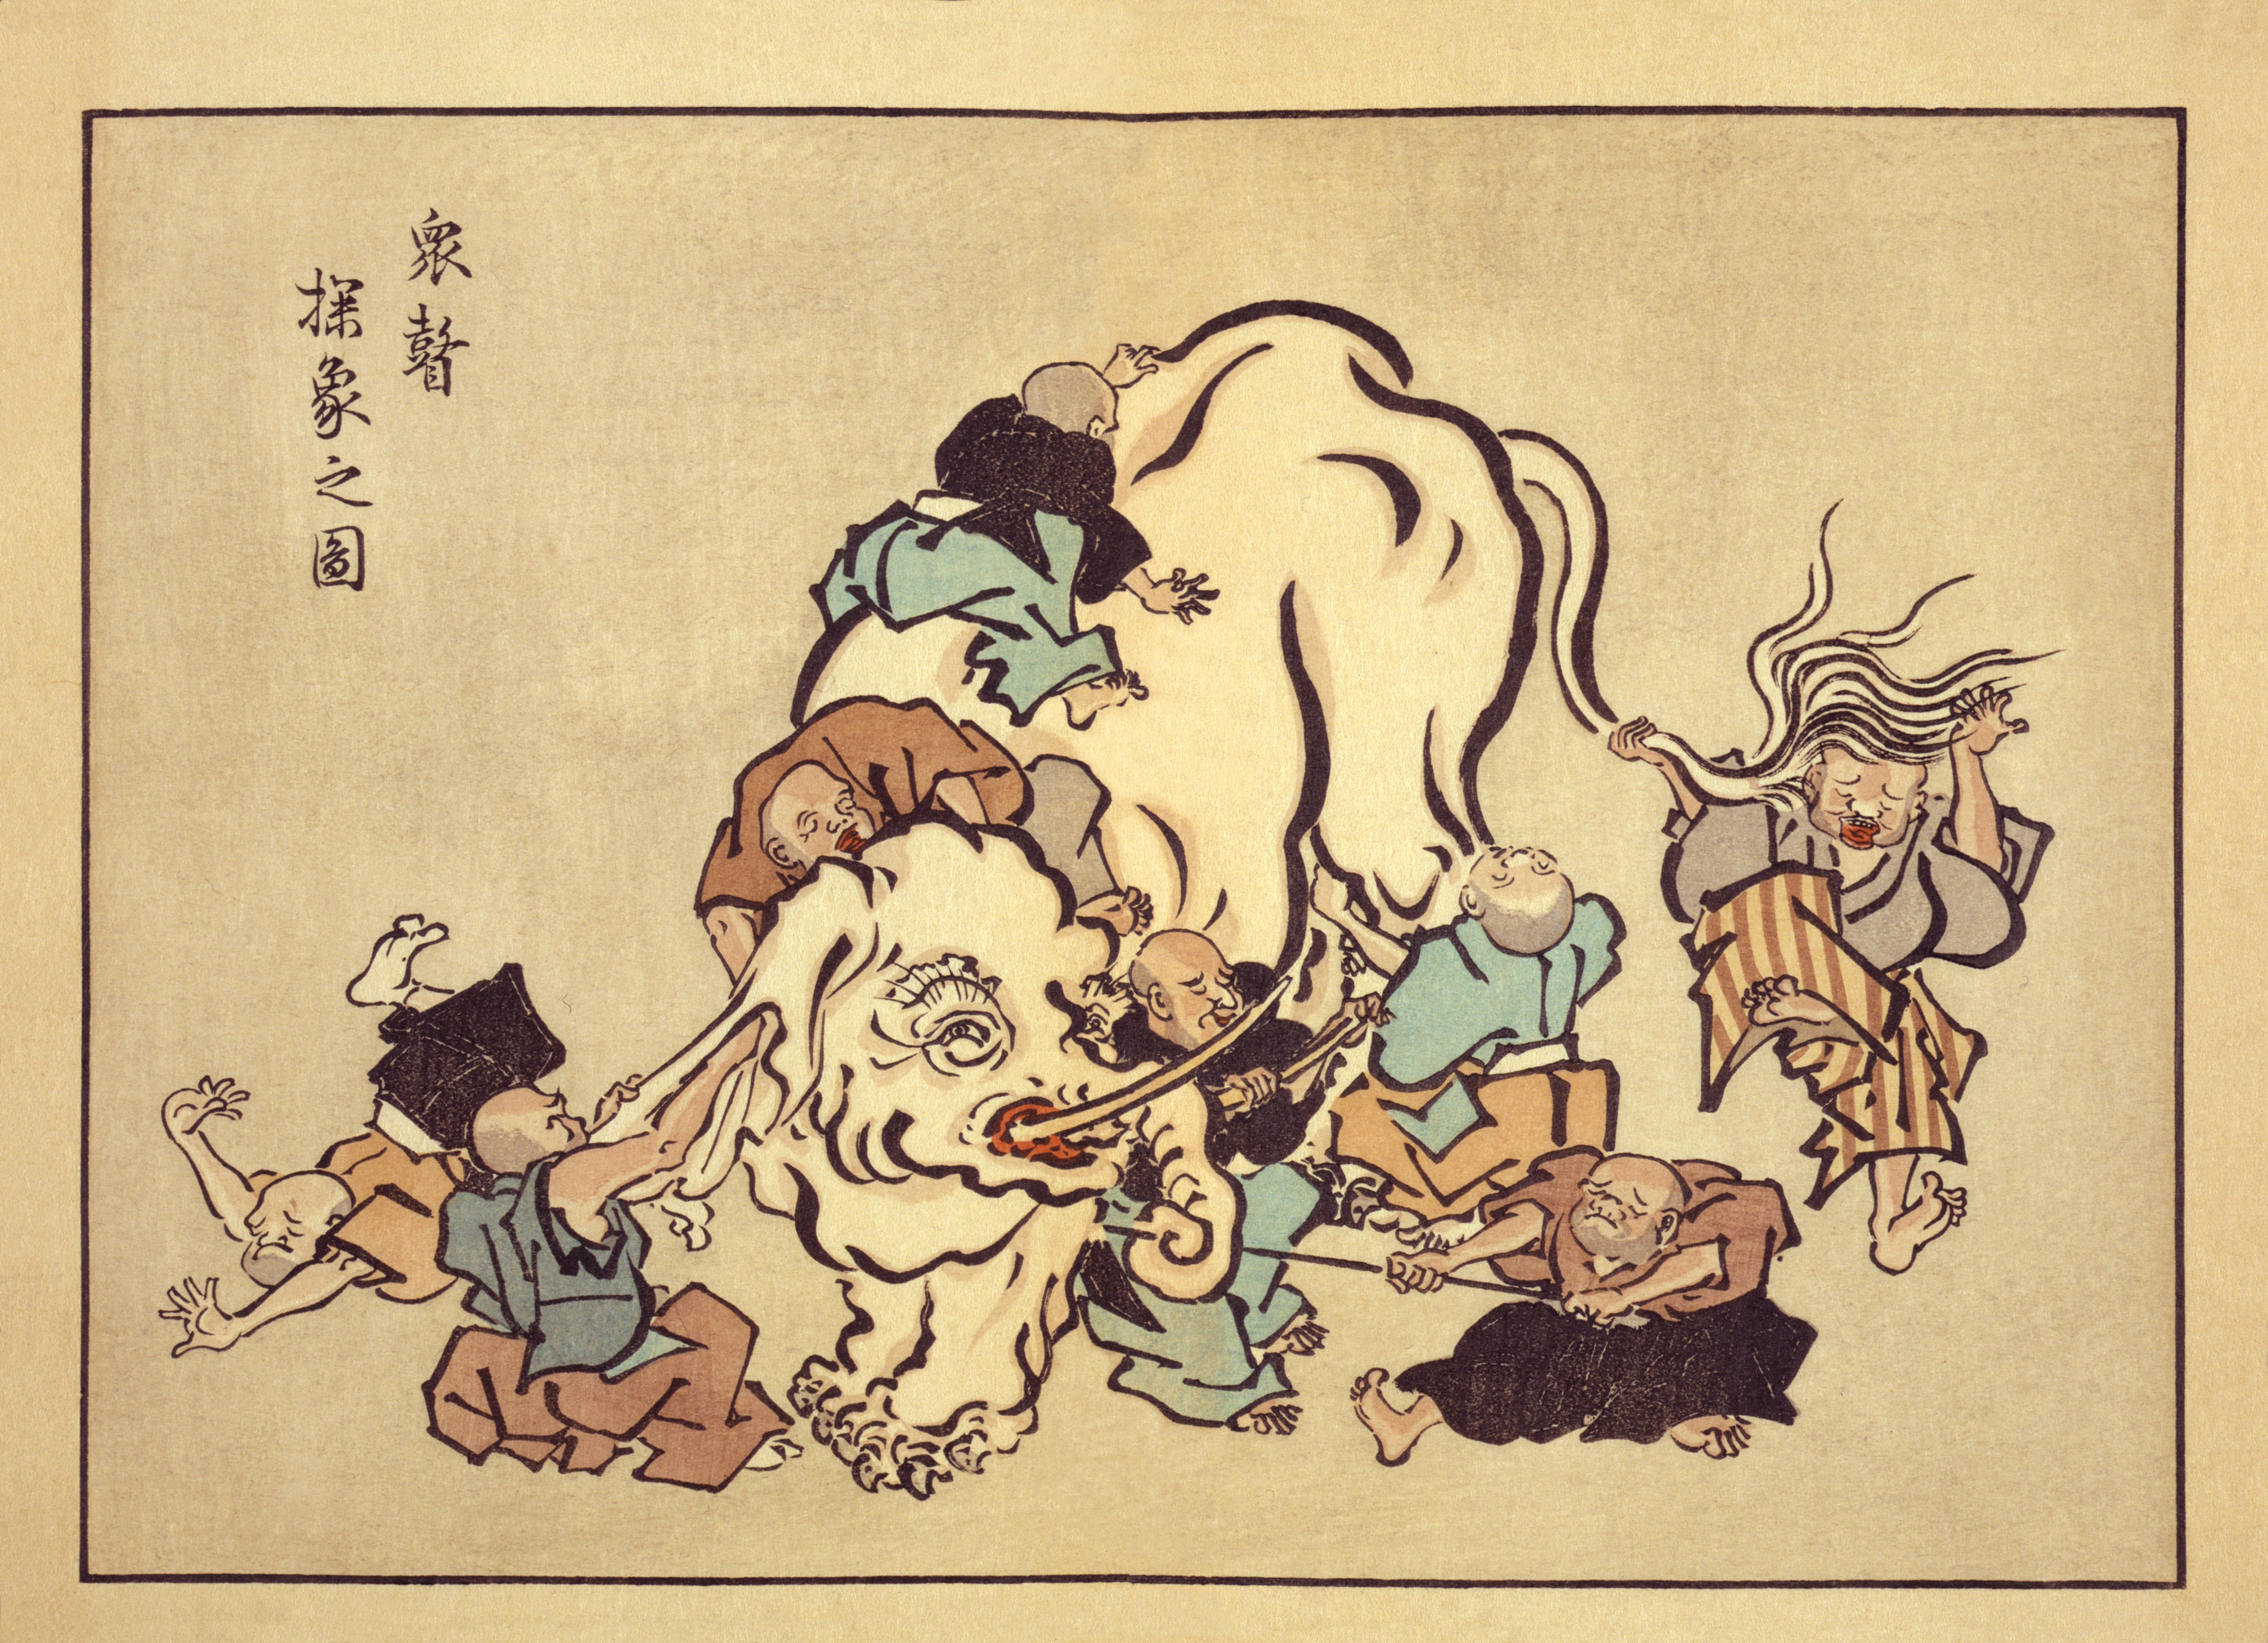
\includegraphics{assets/images/blind-monks.jpg}
  \caption{Blind monks examining the Bitcoin bull}
  \label{fig:blind-monks}
\end{figure}

Bitcoin is a child of many disciplines. Like blind monks examining an elephant,
everyone who approaches this novel technology does so from a different angle.
And everyone will come to different conclusions about the nature of the beast.

The following lessons are about some of my assumptions which Bitcoin shattered,
and the conclusions I arrived at. Philosophical questions of immutability,
scarcity, locality, and identity are explored in the first four lessons.  Every
part consists of seven lessons.

~

\begin{samepage}
Part~\ref{ch:philosophy} -- Philosophy:

\begin{enumerate}
  \item Immutability and change
  \item The scarcity of scarcity
  \item Replication and locality
  \item The problem of identity
  \item An immaculate conception
  \item The power of free speech
  \item The limits of knowledge
\end{enumerate}
\end{samepage}

Lesson \ref{les:5} explores how Bitcoin's origin story is not only fascinating but
absolutely essential for a leaderless system. The last two lessons of this
chapter explore the power of free speech and the limits of our individual
knowledge, reflected by the surprising depth of the Bitcoin rabbit hole.

I hope that you will find the world of Bitcoin as educational, fascinating and
entertaining as I did and still do. I invite you to follow the white rabbit and
explore the depths of this rabbit hole. Now hold on to your pocket watch, pop
down, and enjoy the fall.


\part{Economics}
\label{ch:economics}

\begin{chapquote}{Lewis Carroll, \textit{Alice in Wonderland}}
``A large rose tree stood near the entrance of the garden: the roses on it were
white, but there were three gardeners at it, busily painting them red. This
Alice thought a very curious thing...''
\end{chapquote}

\textit{Money doesn’t grow on trees.} To believe that it does is foolish, and our
parents make sure that we know about that by repeating this saying like a
mantra. We are encouraged to use money wisely, to not spend it frivolously,
and to save it in good times to help us through the bad. Money, after all,
does not grow on trees.

Bitcoin taught me more about money than I ever thought I would need to know.
Through it, I was forced to explore the history of money, banking, various
schools of economic thought, and many other things. The quest to understand
Bitcoin lead me down a plethora of paths, some of which I try to explore in
this series.

In the first seven lessons some of the philosophical questions Bitcoin touches
on were discussed. The next seven lessons will take a closer look at money and
economics.

~

Part II -- Economics:

\begin{enumerate}
  \item Financial ignorance
  \item Inflation
  \item Value
  \item Money
  \item The history and downfall of money
  \item Fractional reserve insanity
  \item Sound money
\end{enumerate}

Again, I will only be able to scratch the surface. Bitcoin is not only
ambitious, but also broad and deep in scope, making it impossible to cover all
relevant topics in a single lesson, essay, article, or book. I  doubt if it is
even possible at all.

\textit{Bitcoin is a new form of money}, which makes learning about
economics paramount to understanding it. Dealing with the nature of human action
and the interactions of economic agents, economics is probably one of the
largest and fuzziest pieces of the Bitcoin puzzle.

Again, these lessons are an exploration of the various things I have learned
from Bitcoin. They are a personal reflection of my journey down the rabbit hole.
Having no background in economics, I am definitely out of my comfort zone and
especially aware that any understanding I might have is incomplete. I will do my
best to outline what I have learned, even at the risk of making a fool out of
myself. After all, I am still trying to answer the question: ``What have you
learned from Bitcoin?''

\begin{figure}
  \centering
  
\includegraphics[width=8cm]{assets/images/the-tweet.png}
  \caption{What have you learned from Bitcoin?}
  \label{fig:the-tweet}
\end{figure}

After seven lessons examined through the lens of philosophy, let’s use the lens
of economics to look at seven more. Economy class is all I can offer this time.
Final destination: \textit{sound money}.

% [the question]: https://twitter.com/arjunblj/status/1050073234719293440

\part{Technology}
\label{ch:technology}

\begin{chapquote}{Lewis Carroll, \textit{Alice in Wonderland}}
``Now, I'll manage better this time'' she said to herself, and began by taking
the little golden key, and unlocking the door that led into the garden
\end{chapquote}

\textit{Golden keys}, clocks which only work by chance, races to solve
strange riddles, and builders that don't have faces or names. What sounds like
fairy tales from Wonderland is daily business in the world of Bitcoin.

As we explored in [Chapter 2][chapter2], large parts of the current financial
system are systematically broken. Like Alice, we can only hope to manage better
this time. But, thanks to a pseudonymous inventor, we have incredibly
sophisticated technology to support us this time around: Bitcoin.

Solving problems in a radically decentralized and adversarial environment
requires unique solutions. What would otherwise be trivial problems to solve
are everything but in this strange world of nodes. Bitcoin relies on strong
cryptography for most solutions, at least if looked at through the lens of
technology. Just how strong this cryptography is will be explored in one of the
following lessons.

\textit{Cryptography} is what Bitcoin uses to remove trust in authorities.
Instead of relying on centralized institutions, the system relies on the final
authority of our universe: physics. Some grains of trust still remain, however.
We will examine these grains in the second lesson of this chapter.

~

Part III -- Technology:

\begin{enumerate}
  \item Strength in numbers
  \item Reflections on \enquote{Don't Trust, Verify}
  \item Telling time takes work
  \item Move slowly and don't break things
  \item Privacy is not dead
  \item Cypherpunks write code
  \item Metaphors for Bitcoin's future
\end{enumerate}

The last couple of lessons explore the ethos of technological development in
Bitcoin, which is arguably as important as the technology itself. Bitcoin is not
the next shiny app on your phone. It is the foundation of a new economic
reality, which is why Bitcoin should be treated as nuclear-grade financial
software.

Where are we in this financial, societal, and technological revolution? Networks
and technologies of the past may serve as metaphors for Bitcoins future, which
are explored in the last lesson of this chapter.

Once more, strap in and enjoy the ride. Like all exponential technologies, we
are about to go parabolic.

\addpart{Final Thoughts}
\pdfbookmark{Conclusion}{conclusion}
\label{ch:conclusion}

\chapter*{Conclusion}

\begin{chapquote}{Lewis Carroll, \textit{Alice im Wunderland}}
\enquote{Begin at the beginning} the King said, very gravely, \enquote{and go on till you
come to the end: then stop.}
\end{chapquote}

As mentioned in the beginning, I think that any answer to the
question \textit{“What have you learned from Bitcoin?”} will always be incomplete. The
symbiosis of what can be seen as multiple living systems -- Bitcoin, the
technosphere, and economics -- is too intertwined, the topics too numerous, and
things are moving too fast to ever be fully understood by a single person.

Even without understanding it fully, and even with all its quirks and seeming
shortcomings, Bitcoin undoubtedly works. It keeps producing blocks roughly every
ten minutes and does so beautifully. The longer Bitcoin continues to work, the
more people will opt-in to use it.

\begin{quotation}\begin{samepage}
\enquote{It's true that things are beautiful when they work. Art is function.}
\begin{flushright} -- Giannina Braschi\footnote{Giannina Braschi, \textit{Empire of Dreams} \cite{braschi2011empire}}
\end{flushright}\end{samepage}\end{quotation}

\paragraph{} Bitcoin is a child of the internet. It is growing exponentially,
blurring the lines between disciplines. It isn’t clear, for example, where the
realm of pure technology ends and where another realm begins. Even though
Bitcoin requires computers to function efficiently, computer science is not
sufficient to understand it. Bitcoin is not only borderless in regards to its
inner workings but also boundaryless in respect to academic disciplines.

Economics, politics, game theory, monetary history, network theory, finance,
cryptography, information theory, censorship, law and regulation, human
organization, psychology -- all these and more are areas of expertise which might
help in the quest of understanding how Bitcoin works and what Bitcoin is.

No single invention is responsible for its success. It is the combination of
multiple, previously unrelated pieces, glued together by game theoretical
incentives, which make up the revolution that is Bitcoin. The beautiful blend of
many disciplines is what makes Satoshi a genius.

\paragraph{} Like every complex system, Bitcoin has to make tradeoffs in terms
of efficiency, cost, security, and many other properties. Just like there is no
perfect solution to deriving a square from a circle, any solution to the
problems which Bitcoin tries to solve will always be imperfect as well.

\begin{quotation}\begin{samepage}
\enquote{I don’t believe we shall ever have a good money again before we take the
thing out of the hands of government, that is, we can’t take it violently
out of the hands of government, all we can do is by some sly roundabout way
introduce something that they can’t stop.}
\begin{flushright} -- Friedrich Hayek\footnote{Friedrich Hayek on Monetary Policy, the Gold Standard, Deficits, Inflation, and John Maynard Keynes \url{https://youtu.be/EYhEDxFwFRU}}
\end{flushright}\end{samepage}\end{quotation}

Bitcoin is the sly, roundabout way to re-introduce good money to the world. It
does so by placing a sovereign individual behind each node, just like Da Vinci
tried to solve the intractable problem of squaring a circle by placing the
Vitruvian Man in its center. Nodes effectively remove any concept of a center,
creating a system which is astonishingly antifragile and extremely hard to shut
down. Bitcoin lives, and its heartbeat will probably outlast all of ours.

I hope you have enjoyed these twenty-one lessons. Maybe the most important
lesson is that Bitcoin should be examined holistically, from multiple angles, if
one would like to have something approximating a complete picture. Just like
removing one part from a complex system destroys the whole, examining parts of
Bitcoin in isolation seems to taint the understanding of it. If only one person
strikes \enquote{blockchain} from her vocabulary and replaces it with \enquote{a
chain of blocks} I will die a happy man.

In any case, my journey continues. I plan to venture further down into the
depths of this rabbit hole, and I invite you to tag
along for the ride.\footnote{\url{https://twitter.com/dergigi}}

% <!-- Twitter -->
% [dergigi]: https://twitter.com/dergigi
%
% <!-- Internal -->
% [sly roundabout way]: https://youtu.be/EYhEDxFwFRU?t=1124
% [Giannina Braschi]: https://en.wikipedia.org/wiki/Braschi%27s_Empire_of_Dreams


\end{document}
